\documentclass{article}
% translate with >> pdflatex -shell-escape <file>

\usepackage{pgfplots}
\pgfplotsset{compat=newest}

\pagestyle{empty}

\begin{document}
\begin{tikzpicture}[scale=1]%
  \begin{axis}[
      width=0.8\textwidth,
      height=0.6\textheight,
      title=Plot of few functions,
      ylabel style={overlay},
      yticklabel style={overlay},
      xlabel={$x$},
      ylabel={$y$},
      %legend style={at={(0.5,0.97)},mark=none,
      %   anchor=north,legend columns=-1},
      legend style={ overlay, at={(-0.4,0.5)}, anchor=center}, every axis plot post/.append style={mark=none},
      domain=2:10,
      ymax=40
   ]
   \addplot {x};
   \addplot {log2(x)};
   \addplot {log2(log2(x))};
   \addplot {x*log2(x)};
   \legend{$x$, $log2(x)$, $log2(log2(x))$, $xlog2(x)$}
   \end{axis}
\end{tikzpicture}%
\end{document}
